\documentclass[titlepage]{article}

\usepackage{
	geometry,
	multicol,
	pdfpages
}

\geometry{
	letterpaper,
	margin=1in
}

\setlength{\columnsep}{0.25in}

\title{
	\textbf{
		CSCE 221 --- 200 \\
		Programming Assignment 4 \\
		Final Report
	}
}

\author{
	James Corder Guy \\
	Nathan Powell
}

\date{
	\today
}

\begin{document}
	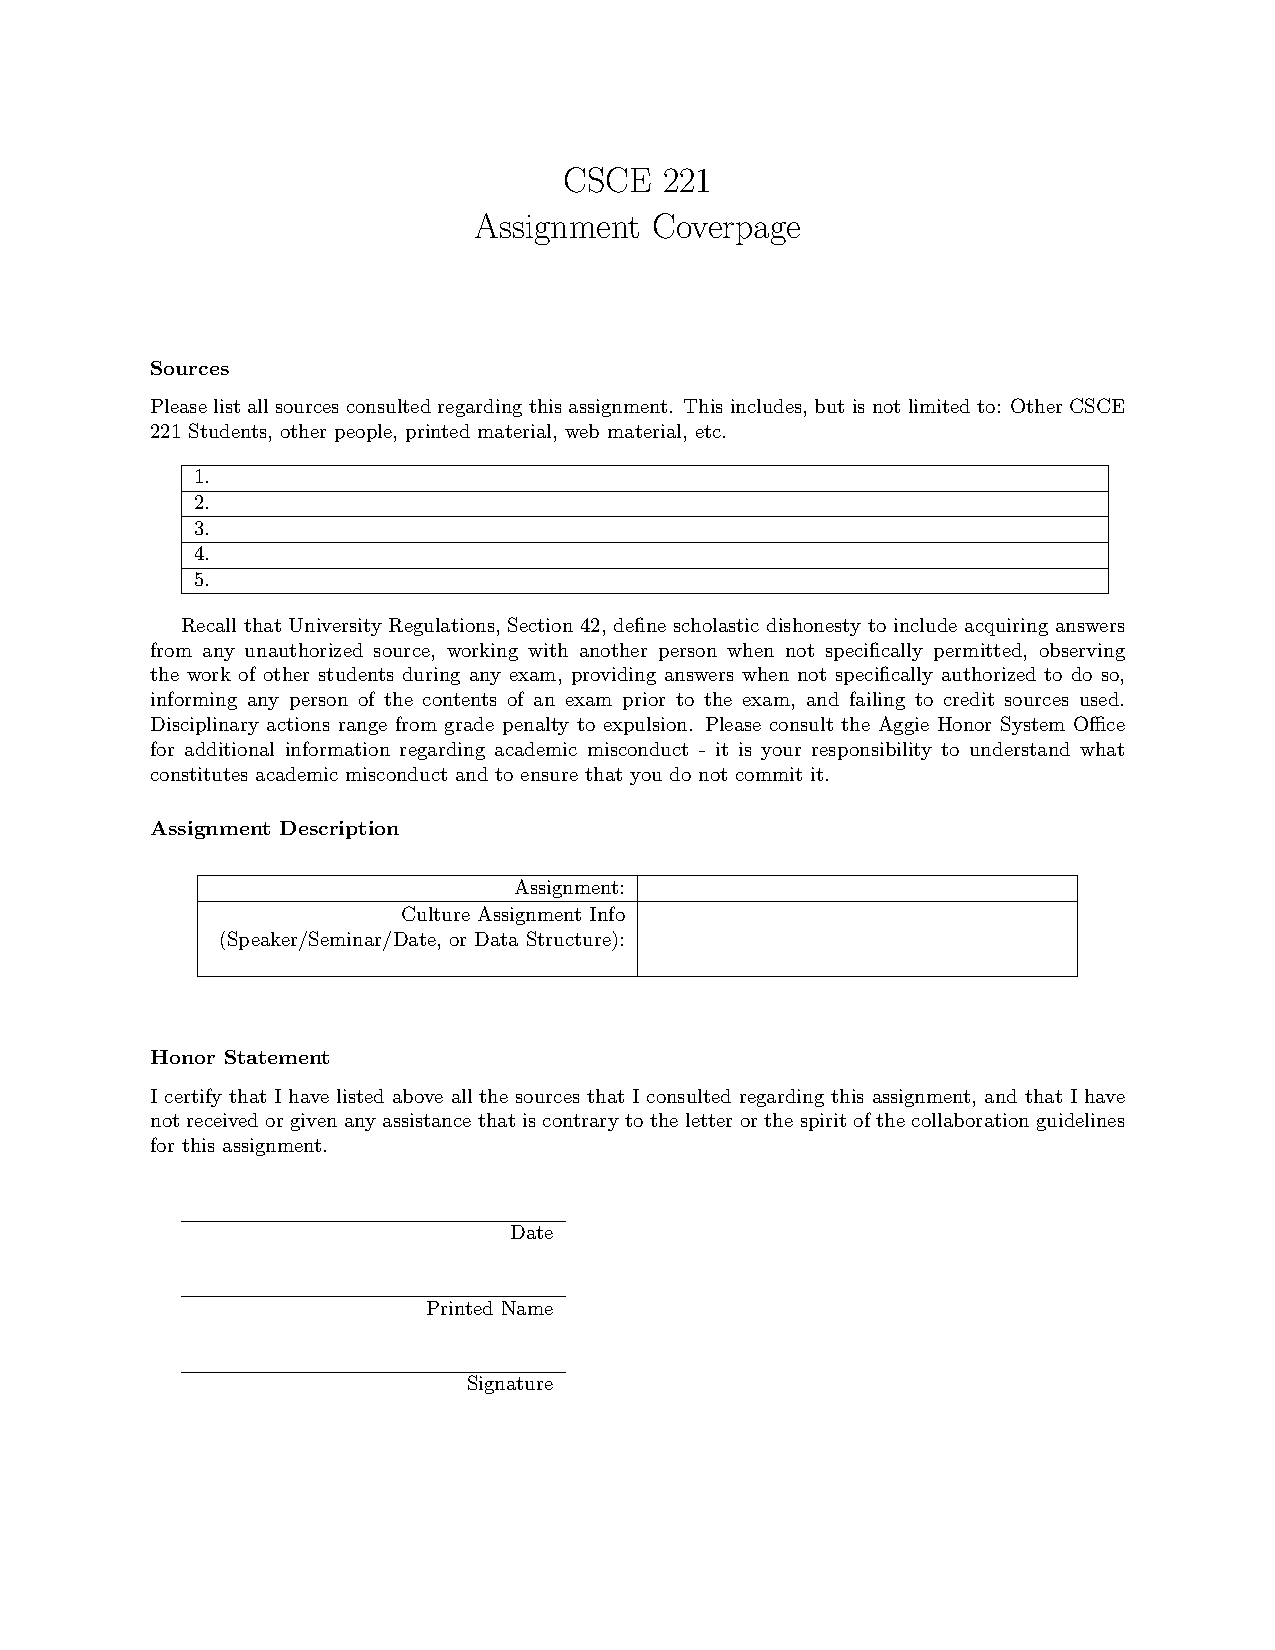
\includepdf[pages={-}]{./coverpage.pdf}
	\maketitle
	\begin{multicols}{2}
		\section{Introduction}
                This report analyzes the implemention of a fully-functional graph data structure, including a searching algorithm and a minimum spanning tree algorithm. [add more once analysis is finished.]
		\section{Implementation Details}
			\subsection{Graph}
                        The graph was implemented using a map of vertices, a master map of edges, and an adjacency edge map for each vertex. The vertex map keys the vertexs by their identifiers, and each element contains a pointer to its respective vertex. Each vertex is assigned a unique identifier number corresponding to the number at which it was inputted, and with a list of edges that connect to it. Both edge maps key the edges by the vertex identifier pairs that they connect, and each element contains a pointer to its respective edge. Each edge is identified by the two vertices it connects, and its weight. All edges are directed; in order to insert an undirected edge, two edges going in opposite directions to the same two vertices are inserted.
			\subsection{Input/Output}
                        The graph pulls its initial vertices and edges from a file, reading in first the number of vertices, then the number of edges. It then reads in the next n lines, where n is the number of vertices, and initializes them as vertices in the vertex container. The graph then reads in the remaining lines as edges, with each line in the order of source vertex, destination vertex, and weight.
			\subsection{Breadth-First Search}
			\subsection{Minimum Spanning Tree}

		\section{Theoretical Analysis}
			\subsection{Graph}
			\subsection{Input/Output}
			\subsection{Breadth-First Search}
			\subsection{Minimum Spanning Tree}

		\section{Experimental Analysis}
			\subsection{Testing Hardware}
			\subsection{Results}
			\subsection{Big-O Constants}
		\section{Results and Discussion}
		\section{Team Contributions}
		\section{Conclusion}
	\end{multicols}
\end{document}
